\documentclass{mmposter}

\colorlet{CEmphasis1}{clustercassis}
\colorlet{CEmphasis2}{clusterblue}

\usepackage{lipsum}
\usepackage{blindtext}
\usepackage{tikz}
\usepackage{amsmath}
\usepackage{hyperref}
\hypersetup{
	colorlinks,
	citecolor=black,
	urlcolor=CEmphasis1,
}

\title{Improving Interoperability\\in Scientific Computing\\via MaRDI Open Interfaces}
\authors{Contributors:
	Dmitry I.\ Kabanov, Stephan Rave, Mario Ohlberger
}
\renewcommand{\refname}{References}

\newcommand{\OIF}{\textsc{MaRDI Open Interfaces}\xspace}

\newcounter{hilfszaehler}

\graphicspath{{./assets/}}

\begin{document}
\bibliographystyle{plain}

\maketitle

\section*{Summary}
We develop \OIF{} to improve interoperability of scientific software.

\begin{objectives}
  \item Develop library that passes data between languages automatically
  \item Develop Open Interfaces for typical numerical problems,
  such as optimization or integration of differential equations
  \item Spread information about Open Interfaces to encourage
  scientific-computing community to program against these interfaces.
\end{objectives}

\section*{Software Architecture and Data Flow}
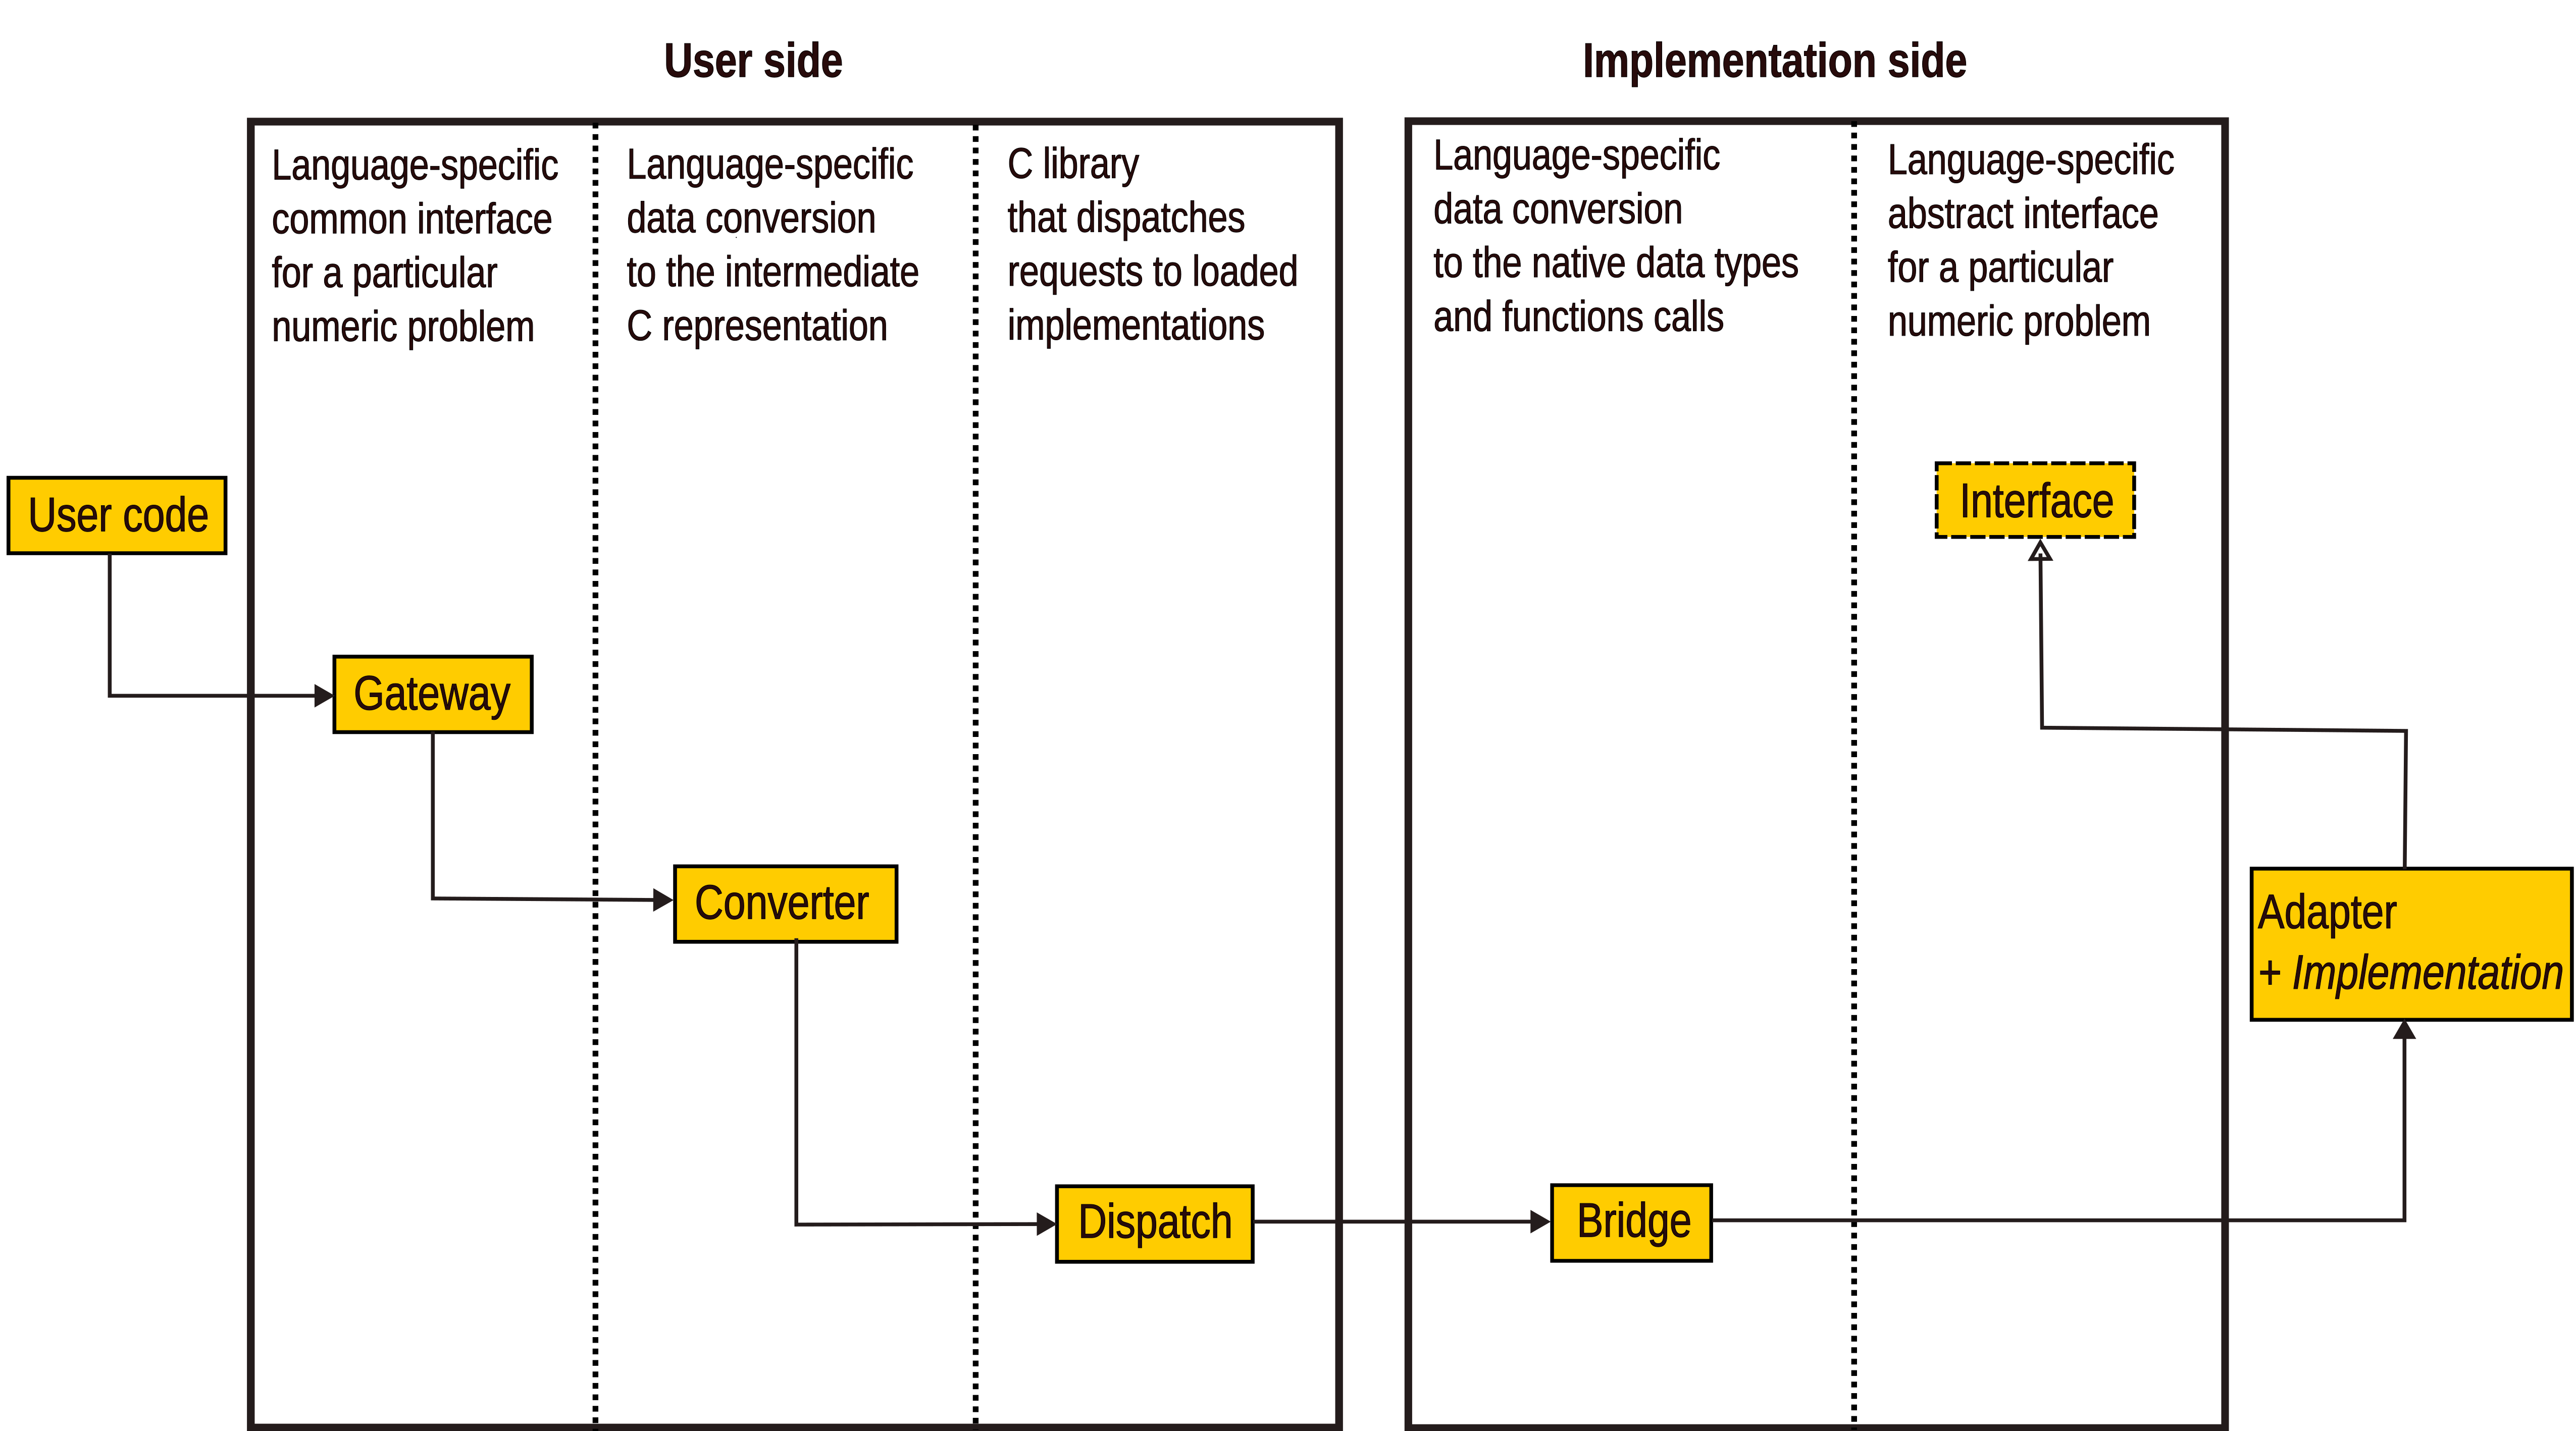
\includegraphics[width=\columnwidth]{arch.png}

\textbf{User} requests an implementation of an Open Interface
and interacts with the implementation only via a \textbf{Gateway},
so that the discrepancies between different implementations in terms
of functions signatures and order of invocation become transparent
to the \textbf{User}.

The function arguments are converted from the user's language
to a C intermediate representation inside a \textbf{Converter}
that passes them further.
The \textbf{Dispatch} is responsible for loading an implementation
and its corresponding runtime (\textbf{Bridge}).
The \textbf{Bridge} converts data from the intermediate representation
to the native data types of the implementation and invokes
the requested function, which also occurs via \textbf{Interface},
that is, the implementation is invoked via an adapter.

\newpage

\section*{Example usage}
\lipsum[2]

\section*{Conclusions}
\lipsum[3]

\section*{Connections to other MaRDI subprojects}

\begin{itemize}[align=left]
  \item[\color{CEmphasis1}M2.3:] Benchmarking of MOR software is potentially
    easier using \OIF{}.
  \item[\color{CEmphasis1}M?.?:] Tool that helps with reproducibility
    by ``containerization''.
\end{itemize}

\begin{thebibliography}{1}
  \setlength{\itemsep}{1pt}
  \setlength{\parskip}{1.5pt}

  \scriptsize{

  \bibitem[1]{PyMOR}
  Ren{\'{e}}, M., Rave, S., and Schindler, F.
  \newblock pyMOR -- Generic Algorithms and Interfaces for Model Order Reduction, 2016.
  \newblock doi:10.1137/15m1026614.
  }
\end{thebibliography}

\end{document}
